% The three sonar types in the sonar simulation design (docs/design/sonar.md), one ping each over a flat seabed.
% Line art in the style of Milne (1983), as in the subsea localization figure.
% (a) imaging sonar: forward multibeam, beams wide in elevation, one image per ping.
% (b) profiling sonar: downward multibeam, beams narrow in both directions, one point per beam, swept by motion.
% (c) sidescan: one beam per side, narrow along track and wide in elevation, one line per ping, swept by motion.
% Build: pdflatex sonar_types.tex, then pdftocairo to ../images/sonar_types.{png,svg}
\documentclass[tikz,border=6pt]{standalone}
\usetikzlibrary{arrows.meta,patterns,calc}
\renewcommand{\familydefault}{\sfdefault}

\tikzset{
  lbl/.style={font=\sffamily\small},
  ttl/.style={font=\sffamily\small,align=center,anchor=south},
  % oblique projection: x forward (right), y to port (into the page), z up
  obl/.style={x={(0.5cm,0cm)},y={(0.3cm,0.24cm)},z={(0cm,0.5cm)}},
  foot/.style={fill=black!15,draw=black},
  old/.style={draw=black!55,densely dashed},
  edge/.style={thin},
  move/.style={thick,-{Latex[length=2.4mm]}},
}

% flat seabed, x from -3.5 to 6.5, y from -5 to 5, with a dotted front edge as in the elevation drawings
\newcommand{\seabed}{
  \draw[fill=white] (-3.5,-5,0) -- (6.5,-5,0) -- (6.5,5,0) -- (-3.5,5,0) -- cycle;
  % explicit dots rather than pattern=dots, which pdftocairo expands into thousands of SVG paths
  \foreach \z [count=\i] in {-0.12,-0.3,-0.48} {
    \pgfmathsetmacro{\o}{mod(\i,2)*0.1}
    \foreach \x in {-3.4,-3.2,...,6.3} \fill ({\x+\o},-5,\z) circle (0.4pt);
    \foreach \y in {-4.75,-4.4,...,4.8} \fill (6.5,{\y+\o*1.4},\z) circle (0.4pt);
  }
  \draw (-3.5,-5,0) -- (-3.5,-5,-0.6) (6.5,-5,-0.6) -- (6.5,5,-0.6);
}

% generic vehicle as a box, origin at the middle of its front face, nose toward +x
\newcommand{\rov}[1]{
  \begin{scope}[shift={#1}]
    \draw[fill=black!15] (-1.4,-0.5,0.35) -- (0,-0.5,0.35) -- (0,0.5,0.35) -- (-1.4,0.5,0.35) -- cycle;   % top
    \draw[fill=white] (-1.4,-0.5,-0.35) -- (0,-0.5,-0.35) -- (0,-0.5,0.35) -- (-1.4,-0.5,0.35) -- cycle; % side
    \draw[fill=white] (0,-0.5,-0.35) -- (0,0.5,-0.35) -- (0,0.5,0.35) -- (0,-0.5,0.35) -- cycle;         % front
  \end{scope}
}

\begin{document}
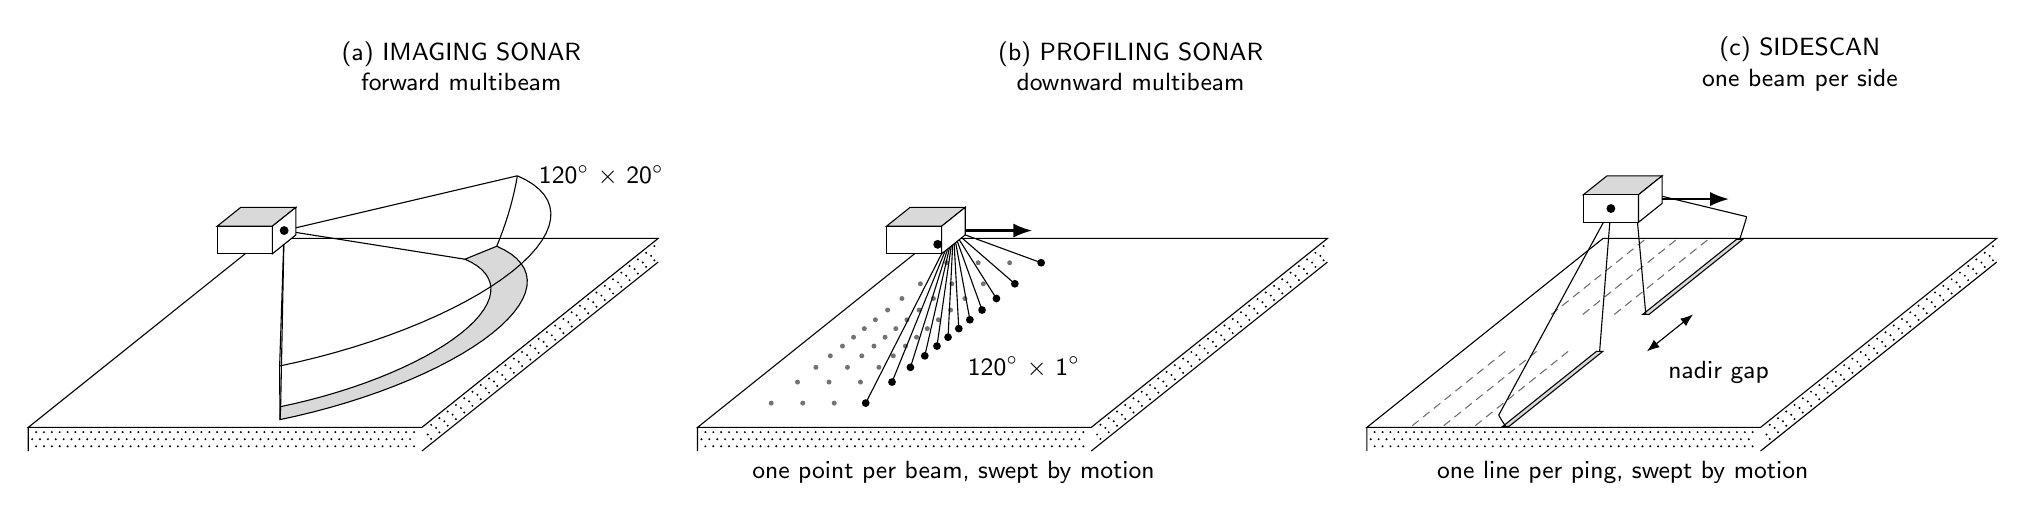
\begin{tikzpicture}[obl]

% ---------------------------------------------------------------- (a) imaging sonar
% head at (0,0,h), tilted down 20 deg; beam 120 deg wide by 20 deg tall (depression 10 to 30 deg); range R
\begin{scope}
  \def\h{2.6}\def\R{5.9}
  \seabed
  \pgfmathsetmacro{\rn}{\h/tan(30)}             % footprint near edge: ground radius at 30 deg depression
  \pgfmathsetmacro{\rf}{sqrt(\R*\R-\h*\h)}      % footprint far edge: limited by range
  \pgfmathsetmacro{\df}{asin(\h/\R)}            % depression at which the range sphere meets the seabed
  \draw[foot] plot[domain=-60:60,samples=31] ({\rn*cos(\x)},{\rn*sin(\x)},0)
          -- plot[domain=60:-60,samples=31] ({\rf*cos(\x)},{\rf*sin(\x)},0) -- cycle;
  % beam edges: lower edge to the seabed, upper edge to range R, joined by the range sphere
  \foreach \a in {-60,60} {
    \draw[edge] (0,0,\h) -- ({\rn*cos(\a)},{\rn*sin(\a)},0);
    \draw[edge] (0,0,\h) -- ({\R*cos(10)*cos(\a)},{\R*cos(10)*sin(\a)},{\h-\R*sin(10)});
    \draw[edge] plot[domain=10:\df,samples=10] ({\R*cos(\x)*cos(\a)},{\R*cos(\x)*sin(\a)},{\h-\R*sin(\x)});
  }
  \draw[edge] plot[domain=-60:60,samples=31] ({\R*cos(10)*cos(\x)},{\R*cos(10)*sin(\x)},{\h-\R*sin(10)});
  \rov{(0,0,\h)}
  \fill (0,0,\h) circle (1.6pt);
  \node[lbl,anchor=west] at ({\R*cos(10)*cos(60)+0.3},{\R*cos(10)*sin(60)},{\h-\R*sin(10)}) {120$^\circ$ $\times$ 20$^\circ$};
  \node[ttl] at (1.5,5,3.5) {(a) IMAGING SONAR\\forward multibeam};
\end{scope}

% ---------------------------------------------------------------- (b) profiling sonar
% head at (0,0,h) pointing down; nominal 120 deg across track by 1 deg along track, beams +-55 deg from nadir; earlier pings behind
\begin{scope}[shift={(17,0,0)}]
  \def\h{2.6}
  \seabed
  \foreach \xo in {-2.4,-1.6,-0.8}
    \foreach \t in {-55,-45,...,55} \fill[black!55] (\xo,{\h*tan(\t)},0) circle (0.9pt);
  \foreach \t in {-55,-45,...,55} {
    \draw[edge] (0,0,\h) -- (0,{\h*tan(\t)},0);
    \fill (0,{\h*tan(\t)},0) circle (1.4pt);
  }
  \rov{(0,0,\h)}
  \fill (-0.4,0,{\h-0.35}) circle (1.6pt);
  \draw[move] (0.3,0,\h) -- (2.0,0,\h);
  \node[lbl,anchor=north] at (3,-5,-0.6) {one point per beam, swept by motion};
  \node[lbl,anchor=west] at (1.2,-1.8,0) {120$^\circ$ $\times$ 1$^\circ$};
  \node[ttl] at (1.5,5,3.5) {(b) PROFILING SONAR\\downward multibeam};
\end{scope}

% ---------------------------------------------------------------- (c) sidescan
% vehicle at height h, transducer on each side at y=+-0.5; one beam per side, 0.5 deg along track,
% depression 32 to 82 deg (50 deg tall), range R
\begin{scope}[shift={(34,0,0)}]
  \def\h{3.4}\def\R{5.6}
  \seabed
  \pgfmathsetmacro{\yn}{0.5+\h/tan(82)}         % inner edge of each swath
  \pgfmathsetmacro{\yf}{0.5+sqrt(\R*\R-\h*\h)}  % outer edge, limited by range
  \pgfmathsetmacro{\df}{asin(\h/\R)}
  % earlier pings, then this ping
  \foreach \xo in {-2.4,-1.6,-0.8}
    \foreach \s in {-1,1} \draw[old] (\xo,{\s*\yn},0) -- (\xo,{\s*\yf},0);
  \foreach \s in {-1,1} {
    \draw[foot] (-0.08,{\s*\yn},0) -- (0.08,{\s*\yn},0) -- (0.08,{\s*\yf},0) -- (-0.08,{\s*\yf},0) -- cycle;
    \draw[edge] (0,{\s*0.5},\h) -- (0,{\s*\yn},0);
    \draw[edge] (0,{\s*0.5},\h) -- (0,{\s*(0.5+\R*cos(32))},{\h-\R*sin(32)});
    \draw[edge] plot[domain=32:\df,samples=10] (0,{\s*(0.5+\R*cos(\x))},{\h-\R*sin(\x)});
  }
  \draw[{Latex[length=1.6mm]}-{Latex[length=1.6mm]}] (1.2,{-\yn},0) -- (1.2,{\yn},0);
  \node[lbl,anchor=north west] at (1.5,{-\yn},0) {nadir gap};
  \rov{(0.7,0,\h)}
  \fill (0,-0.5,\h) circle (1.6pt);
  \draw[move] (1.0,0,\h) -- (2.7,0,\h);
  \node[lbl,anchor=north] at (3,-5,-0.6) {one line per ping, swept by motion};
  \node[ttl] at (1.5,5,3.5) {(c) SIDESCAN\\one beam per side};
\end{scope}

\end{tikzpicture}
\end{document}
